\documentclass[10pt]{beamer}

\mode<presentation> {

% \usetheme{Berlin}  % Squares
\usetheme{Madrid}  % Circles & dense
% \usetheme{Frankfurt}  % Cirles

\setbeamertemplate{headline}{%
\leavevmode%
  \hbox{%
    \begin{beamercolorbox}[wd=\paperwidth,ht=2.5ex,dp=1.125ex]{palette quaternary}%
    \insertsectionnavigationhorizontal{\paperwidth}{}{\hskip0pt plus1filll}
    \end{beamercolorbox}%
  }
}

\setbeamertemplate{navigation symbols}{}  % To remove the navigation symbols from the bottom of all slides uncomment this line
\setbeamertemplate{items}[circle]

% \useoutertheme{miniframes}
% \useinnertheme{circles}

}

\usepackage{graphicx}
\usepackage{booktabs}
\usepackage{fontspec}
\usepackage{xunicode}
\usepackage{tabularx}
\usepackage{xltxtra}
\usepackage{xecyr}
\usepackage{hyperref}
\usepackage{amsthm}
\usepackage{blindtext}
\usepackage{color}
\usepackage[normalem]{ulem}
\usepackage{url}
\usepackage[font=small,labelfont=bf]{caption}
\usepackage[subrefformat=parens]{subcaption}
\captionsetup{compatibility=false}
\captionsetup[subfigure]{labelformat=empty}
\captionsetup[figure]{labelformat=empty}

\usepackage{polyglossia}
\setdefaultlanguage{russian}
\setmainfont[Mapping=tex-text]{CMU Serif}
\setsansfont[Mapping=tex-text]{CMU Sans Serif}
\setmonofont[Mapping=tex-text]{CMU Serif}

\makeatletter
\DeclareUrlCommand\ULurl@@{%
  \def\UrlFont{\ttfamily\color{blue}}%
  \def\UrlLeft{\uline\bgroup}%
  \def\UrlRight{\egroup}}
\def\ULurl@#1{\hyper@linkurl{\ULurl@@{#1}}{#1}}
\DeclareRobustCommand*\ULurl{\hyper@normalise\ULurl@}
\makeatother

\newcommand\TODO[1]{\textcolor{red}{{\Large TODO: #1}}}
\newcommand\NaN{\textcolor{red}{NaN}}

%-------------------------------------------------------------------------------
%	TITLE PAGE
%-------------------------------------------------------------------------------

\title[Определение наилучшего ответа на SO]{Определение наилучшего ответа на StackOverflow}
\author[Никита Подгузов]{
Никита Подгузов 
\texorpdfstring{\vskip0.5cm \footnotesize{Научный руководитель: Рауф Курбанов}}{}
}
\institute[СПбАУ]{Санкт-Петербургский Академический университет}
\date{18 июня 2018 года}
\begin{document}

%-------------------------------------------------------------------------------
%	PRESENTATION SLIDES
%-------------------------------------------------------------------------------

\begin{frame}
\titlepage
\end{frame}

%-------------------------------------------------------------------------------

\begin{frame}
\frametitle{Введение}
\framesubtitle{Обзор}

\begin{columns}
    \begin{column}{0.6\textwidth}
        Возможности сервисов вопросов и ответов:
        \begin{itemize}
            \item Задавать вопрос (и отмечать правильный ответ) 
            \item Отвечать на вопросы, заданные другими пользователями
            \item Голосовать за понравившиеся ответы
        \end{itemize}
    \end{column}
    \begin{column}{0.4\textwidth}
        \begin{center}
            
\includegraphics[width=0.7\textwidth]{images/yahoo_answers_logo.png} \\
            
\includegraphics[width=0.7\textwidth]{images/quora_logo.png} \\
            
\includegraphics[width=0.7\textwidth]{images/stackoverflow_logo.png}
        \end{center}
    \end{column}
\end{columns}
\end{frame}

%-------------------------------------------------------------------------------

\begin{frame}
\frametitle{Введение}
\framesubtitle{ServerFault}

\begin{columns}
    \begin{column}{0.4\textwidth}
    	Особенности системы:
    	\begin{itemize}
			\item Узкоспециализированная
			\item Большая база вопросов
    	\end{itemize}
    \end{column}
    \begin{column}{0.6\textwidth}
        \begin{center}
            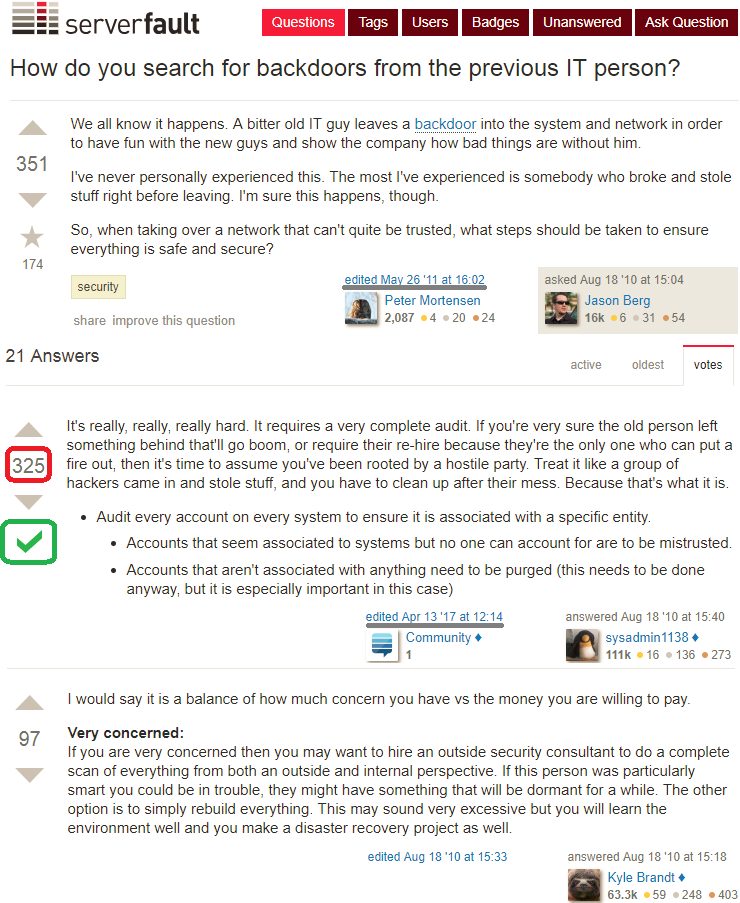
\includegraphics[width=0.8\textwidth]{images/serverfault_screen.png}
        \end{center}
    \end{column}
\end{columns}

\end{frame}

%-------------------------------------------------------------------------------

\begin{frame}
\frametitle{Введение}
\framesubtitle{Постановка задачи}

Проблемы:
\begin{itemize}
	\item Большая доля "неразрешенных" вопросов
	\item Нет возможности помочь оценить правильность ответов пользователю, задавшему новый вопрос
\end{itemize}

\vskip0.5cm

Хотим научиться определять правильные ответы, используя базу вопросов ServerFault

\end{frame}

%-------------------------------------------------------------------------------

\begin{frame}
\frametitle{Актуальность}
\framesubtitle{Google \& StackOverflow}

\begin{figure}
	\begin{subfigure}[b]{0.49\linewidth}
		\centering
		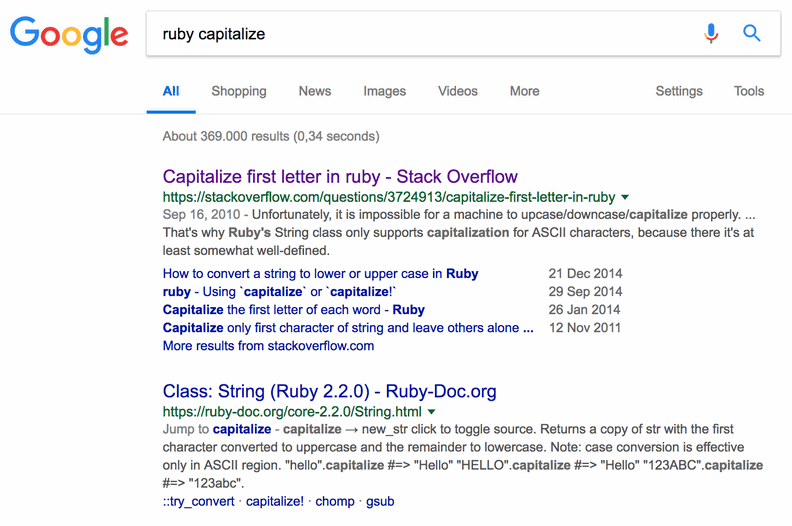
\includegraphics[width=\linewidth]{images/google_search_old.png}
		\caption{Старая версия}
	\end{subfigure}\hfill
	\begin{subfigure}[b]{0.49\linewidth}
		\centering
		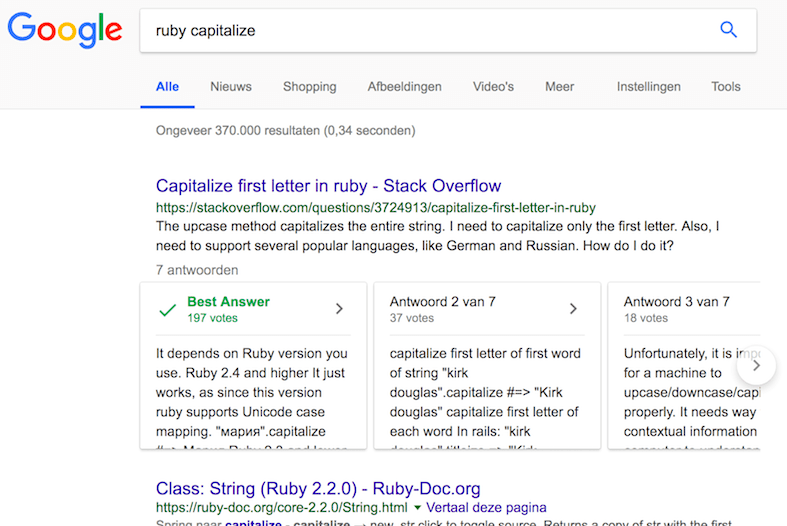
\includegraphics[width=\linewidth]{images/google_search_new.png}
		\caption{Новая версия}
	\end{subfigure}
\end{figure}

\end{frame}

%-------------------------------------------------------------------------------

\begin{frame}
\frametitle{Введение}
\framesubtitle{Обзор имеющихся решений}

\begin{itemize}
	\setlength{\itemsep}{1em}

	\item Burel et al. (2012)
	
	"Automatic Identification of Best Answers in Online Enquiry Communities" 

	\item Tian et al. (2013) 
	
	"Towards Predicting the Best Answers in Community-Based Question-Answering Services" 

	\item Gkotsis et al. (2014)
	
	"It’s all in the Content: State of the art Best Answer Prediction based on Discretisation of Shallow Linguistic Features"

\end{itemize}

\end{frame}

%-------------------------------------------------------------------------------

\begin{frame}
\frametitle{Введение}
\framesubtitle{Обзор имеющихся решений}

\begin{itemize}
	\item Тестирование проводилось на данных ServerFault
	\item Виды фичей: $A \leftrightarrow A$, $A \leftrightarrow Q$, $A$, $user/answer-rating$, $thread$ 
	\item Лингвистических фичи (длина текста, количество предложений, читаемость и др.)
	\item Vector Space Model + TF-IDF для определения похожести
	\item Вероятностная униграмная модель для оценки вероятности ответа
	\item Группировка ответов и дискретизация фичей
	\item Не учитывается наличие сниппетов кода
	\item Alternating Decision Tree / Random Forest Classifier
\end{itemize}

\end{frame}

%-------------------------------------------------------------------------------

\begin{frame}
\frametitle{Введение}
\framesubtitle{Минусы имеющихся решений}

\begin{itemize}
	\setlength{\itemsep}{1em}
	\item Не используется текст вопроса
	\item Не учитывается контекст слова в предложении
	\item Игнорируется семантика
\end{itemize}

\end{frame}


%-------------------------------------------------------------------------------

\begin{frame}
\frametitle{Цель и задачи}

Цель: Научиться определять правильность ответа на StackOverflow, используя тексты вопроса и ответов

\medskip

Задачи:
\begin{itemize}
	\item Произвести сбор данных для обучения и тестирования
	\item Реализовать несколько моделей классификаторов на основе нейронных сетей, использующих тексты ответов
	\item Улучшить точность классификации за счет текста вопроса
	\item Сравнить результаты с имеющимися работами
\end{itemize}


\end{frame}

%-------------------------------------------------------------------------------

\begin{frame}
\frametitle{Данные}
\framesubtitle{Общие факты}

Данные:

\begin{itemize}
	\item База вопросов ServerFault
	\item \texttt{XML}-файл размером $\sim0.9GB$
	\item Новые данные могут быть получены с помощью \texttt{API}
	\item Формат файла: $type\_id$, $id$, $score$, $date$, $body$
\end{itemize}

\end{frame}

%-------------------------------------------------------------------------------

\begin{frame}
\frametitle{Данные}
\framesubtitle{Анализ и обработка}

Анализ:

\begin{itemize}
	\item $684$ тысячи постов, из них $257$ тысяч вопросов и $427$ тысяч ответов
	\item $130$ тысяч вопросов $(51\%)$ без отмеченного правильного ответа
	\item $28$ тысяч вопросов $(11\%)$, у которых нет ни одного ответа
	\item Большое количество технических терминов и слов с опечатками
\end{itemize}

После обработки получили $80$ тысяч вопросов и $180$ тысяч ответов

\end{frame}

%-------------------------------------------------------------------------------

\begin{frame}
\frametitle{Данные}
\framesubtitle{Извлечение признаков}

Признаки:

\begin{itemize}
	\item Векторные представления вопроса и ответа
	\item Лингвистические: количество ссылок, параграфов, сниппетов кода, длина текста, средняя длина предложения, различные индексы удобочитаемости
	\item $thread$: позиция ответа, относительная позиция ответа
\end{itemize}

\end{frame}

%-------------------------------------------------------------------------------

\begin{frame}
\frametitle{Подходы к представлению текста}

\begin{columns}
    \begin{column}{0.5\textwidth}
		\begin{itemize}
			\item
			Bag of words

			Минусы: не учитывается порядок слов и семантика, большая размерность

			\item
			Word2Vec
	
			Обучение на неразмеченном корпусе текстов, для каждого слова получаем вектор, отражающий его семантику.

			Минусы: не дает векторное представления для слов не из словаря

			\item
			Fasttext

			Модификация Word2Vec, основанная на работе с $n$-грамммами букв
		\end{itemize}
	\end{column}
    \begin{column}{0.5\textwidth}
        \begin{center}
        	\begin{figure}
	            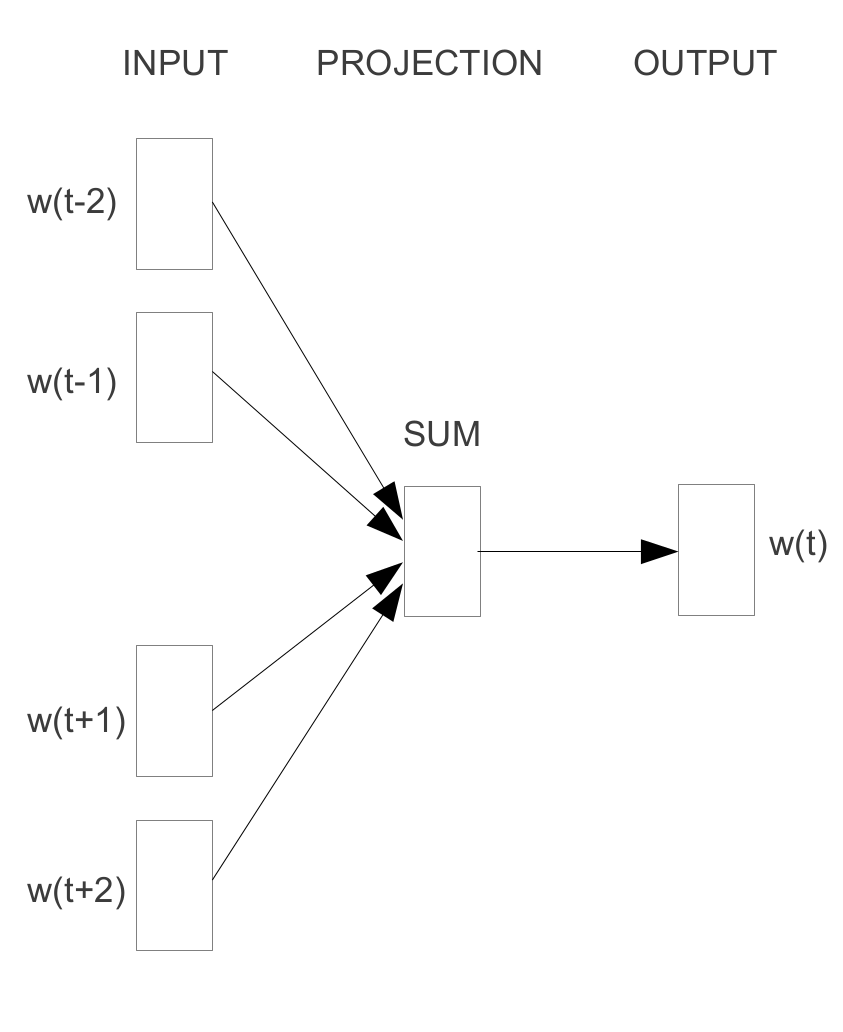
\includegraphics[width=0.9\textwidth]{images/cbow.png} 
    	        \caption{Архитектура модели CBOW}
        	\end{figure}
        \end{center}
    \end{column}
\end{columns}

\end{frame}

%-------------------------------------------------------------------------------

\begin{frame}
\frametitle{Решение задачи}
\framesubtitle{Сверточная нейронная сеть}

\begin{figure}
	\centering
	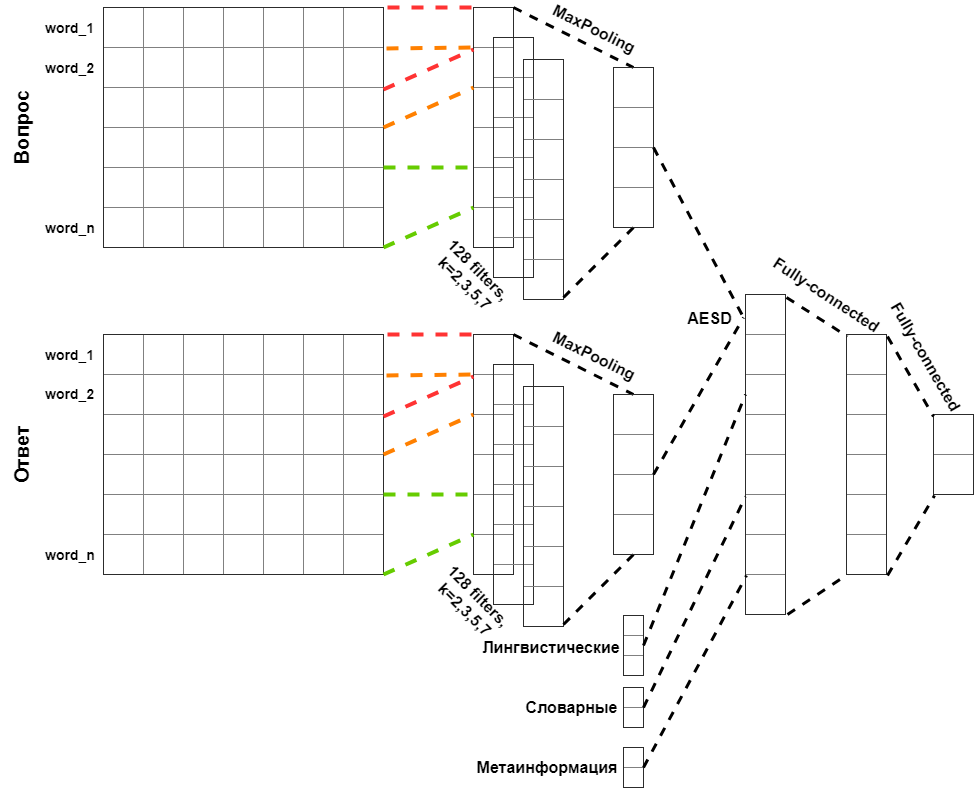
\includegraphics[width=0.7\linewidth]{images/my_cnn.png}
\end{figure}

\end{frame}

%-------------------------------------------------------------------------------

\begin{frame}
\frametitle{Решение задачи}
\framesubtitle{Рекуррентная нейронная сеть}

\begin{figure}
	\centering
	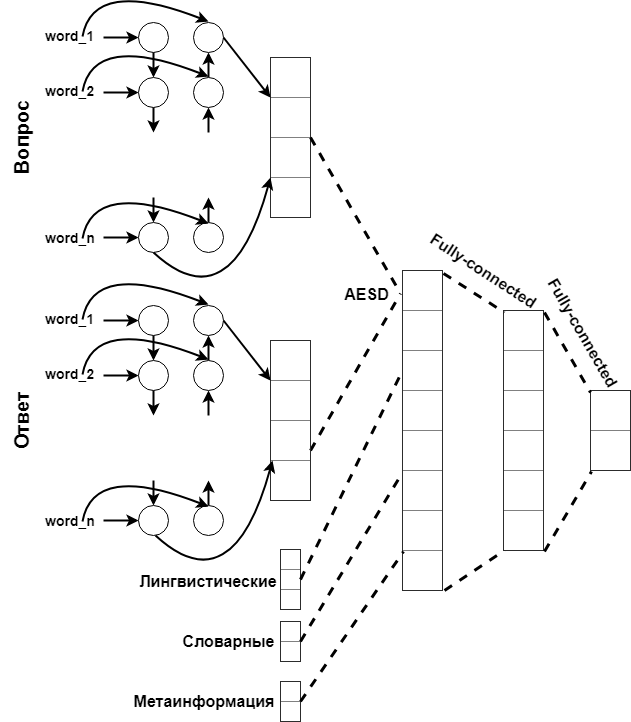
\includegraphics[width=0.5\linewidth]{images/my_rnn.png}
\end{figure}

\end{frame}

%-------------------------------------------------------------------------------

\begin{frame}
\frametitle{Результаты}

\begin{center}
	\small
    \begin{tabularx}{\textwidth}{| l | X | l | l | l | l | l |}
        \hline
	    \textbf{Модель} & \textbf{Виды признаков} & $\mathbf{Acc}$ & $\mathbf{P}$ & $\mathbf{R}$ & $\mathbf{F_1}$ & $\mathbf{AUC}$ \\ \hline
        \hline
	    First-answer & метаинформация & 0.66 & 0.69 & 0.60 & 0.64 & 0.66 \\ \hline
    	Naive-Bayes with TF-IDF & словарные & 0.6 & 0.58 & 0.54 & 0.56 & 0.59 \\ \hline
        \hline
	    Burel et al. (2012) & лингвистические, словарные, пользовательские, метаинформация & - & 0.77 & 0.77 & 0.76 & 0.83 \\ \hline
    	Tian et al. (2013) & лингвистические, метаинформация & 0.72 & - & - & - & - \\ \hline
        Gkotsis et al. (2014) & лингвистические, словарные, метаинформация & - & 0.83 & 0.66 & 0.74 & 0.85 \\ \hline
	    \hline
        CNN & лингвистические, текстовые, метаинформация & \textbf{0.77} & 0.81 & 0.62 & 0.71 & \textbf{0.86} \\ \hline
	    RNN & лингвистические, текстовые, метаинформация & \textbf{0.78} & 0.82 & 0.64 & 0.72 & \textbf{0.87} \\ \hline
    \end{tabularx}
\end{center}
\end{frame}

%-------------------------------------------------------------------------------

\begin{frame}
\frametitle{Выводы}

\begin{itemize}
	\item Подготовлен корпус данных, представляющий из себя ответы на вопросы с сайта Server Fault
	\item Реализовано несколько различных архитектур нейронных сетей для решения задачи определения наилучшего ответа на StackOverflow
	\item Показано, что текст вопроса является важным признаком для классификации
	\item Полученные результаты свидетельствуют о том, что нейронные сети справляются с задачей лучше методов, использованных в других статьях
\end{itemize}

\end{frame}


%-------------------------------------------------------------------------------
%	END PRESENTATION SLIDES
%-------------------------------------------------------------------------------

\end{document}